\documentclass[times, utf8, zavrsni]{fer}
\usepackage{booktabs}
\usepackage{graphicx}
% -- Loading the code block package:
\usepackage{listings}% -- Basic formatting
\setlength{\parindent}{8pt}
\usepackage{indentfirst}% -- Defining colors:
\usepackage[dvipsnames]{xcolor}
\usepackage{caption}
\usepackage{amsmath}
\usepackage{amsfonts}
\usepackage{amssymb}
\definecolor{codegreen}{rgb}{0,0.6,0}
\definecolor{codegray}{rgb}{0.5,0.5,0.5}
\definecolor{codepurple}{rgb}{0.58,0,0.82}
\definecolor{backcolour}{rgb}{1,1,1}% Definig a custom style:
\lstdefinestyle{mystyle}{
    backgroundcolor=\color{backcolour},   
    commentstyle=\color{codepurple},
    keywordstyle=\color{NavyBlue},
    numberstyle=\tiny\color{codegray},
    stringstyle=\color{codepurple},
    basicstyle=\ttfamily\footnotesize\bfseries,
    breakatwhitespace=false,         
    breaklines=true,                 
    captionpos=t,                    
    keepspaces=true,                 
    numbers=left,                    
    numbersep=5pt,                  
    showspaces=false,                
    showstringspaces=false,
    showtabs=false,                  
    tabsize=2
}% -- Setting up the custom style:
\lstset{style=mystyle}

\definecolor{light-gray}{gray}{0.95}
\newcommand{\code}[1]{\colorbox{light-gray}{\texttt{#1}}}
\newcommand{\source}[1]{\caption*{Source: {#1}} }
\usepackage{pdfpages}

\begin{document}

% TODO: Navedite broj rada.
\thesisnumber{1102}

% TODO: Navedite naslov rada.
\title{Klasifikacija prometnih znakova}

% TODO: Navedite vaše ime i prezime.
\author{Matija Pavlović}

\maketitle

% Ispis stranice s napomenom o umetanju izvornika rada. Uklonite naredbu \izvornik ako želite izbaciti tu stranicu.

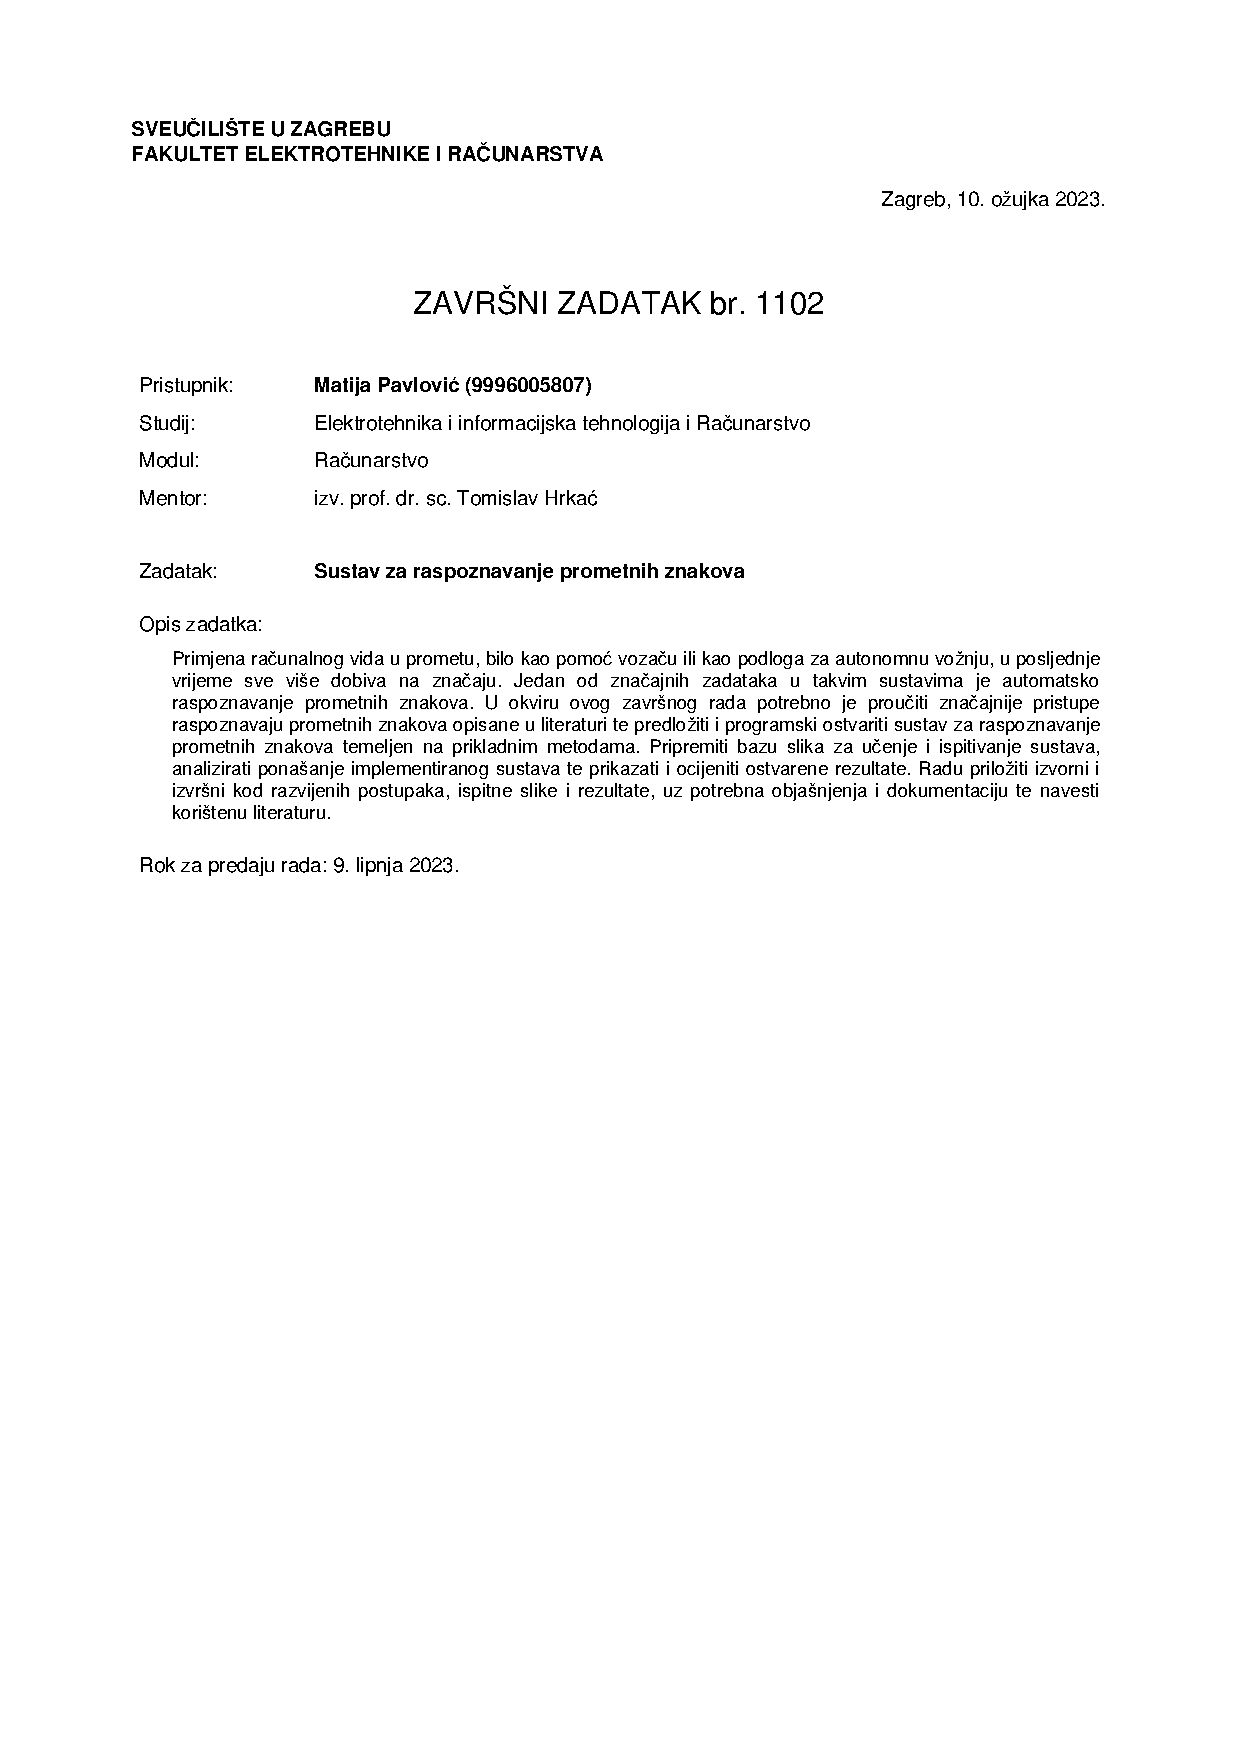
\includepdf[page=-]{izvornik}
% Dodavanje zahvale ili prazne stranice. Ako ne želite dodati zahvalu, naredbu ostavite radi prazne stranice.
\zahvala{}

\tableofcontents

\chapter{Uvod}
Razvoj tehnologije u automobilskoj industriji u stopu prate i sve veći zahtjevi tržišta za novim sigurnosnim značajkama te značajkama koje doprinose udobnosti korištenja vozila. Novi modeli vozila tako postaju opremljeni značajnim brojem senzora na vanjskoj strani vozila i značajnim brojem ekrana i signalnih lampica u unutrašnjosti vozila. Kada sjednemo za upravljač novijih vozila sve češće možemo primijetiti da nas vozilo upozorava na prometne znakove, primjerice ograničenja brzine, zabrane pretjecanja, znakove obaveznog zaustavljanja itd. Razmotrimo li i činjenicu da ubrzano raste i broj vozila s određenim stupnjem autonomije pri vožnji postaje jasno da su sustavi koji u stvarnom vremenu detektiraju i klasificiraju prometne znakove postali izrazito važni u razvoju novih modela vozila. Cilj ovog završnog rada je demonstracija rada jednog takvog sustava uz detaljni opis primjene, problema s kojima se sustav može suočavati u stvarnim okolnostima, te opis implementacije sustava. U sklopu rada ću razviti model strojnog učenja temeljen na dubokoj konvolucijskoj mreži, obraditi skup podataka za treniranje i testiranje modela, te programski kod koji će koristiti kameru prijenosnog računala kako bi klasificirao prometne znakove.

\chapter{Pregled postojeće literature}
Klasifikacija prometnih znakova nije nov pojam u području računarske znanosti i specifičnije području računalnog vida. Shodno tome postoji velik broj znanstvenih radova koji se bave tom problematikom.
Većina pristupa problemu klasifikacije se bazira na pristupu usmjerenom na prepoznavanje boja i oblika \citep{6033494}.
Uz klasifikaciju prometnih znakova se često veže i pojam detekcije.
Kad razmatramo klasifikatore koji su učestalo korišteni pri izradi sustava za detekciju prometnih znakova pronalazimo širok spektar metoda. 
U prvom redu se ističu neuronske mreže, metode potpornih vektora, u hrvatskoj literaturi poznata i kao metoda jezgrenih funkcija, konvolucijske neuronske mreže, nasumične šume, metoda najbližih susjeda...
Iz ovog skupa klasifikatora se za zadaće klasifikacije ipak najčešće koriste konvolucijske neuronske mreže \citep{9065537}.
Ciresan, Meier, Masci i Schmidhuber su pak izbjegli korištenea pretpostavljenih ekstraktora značajki i zamjenili ih postupcima nadziranog učenja. Kombinacijom raznih dubokih
neuronskih mreža treniranih na različito pretprocesiranim podatcima ostvarili su MCDNN, odnosno višestupčanu neuronsku mrežu, tako ostvarivši sustav koji je otporan na varijacije u kontrastu i osvjetljenju \citep{CIRESAN2012333}.
\chapter{Metodologija rada}
U poglavlju metodologija rada opisati ću metode pri izradi projekta od razine prikupljanja i prilagodbe podataka za treniranje modela strojnog učenja, kreiranje samog modela, treniranje modela te naposlijetku i izradu testne aplikacije kojom se demonstrira rad sustava.
Isto tako detaljno ću opisati i arhitekturu same duboke neuronske mreže, argumentirati izbor aktivacijskih funkcija korištenih na izlazima iz slojeva neuronske mreže, odabir optimizatora te odabir metode za proračun pogreške predikcije modela.
\pagebreak
\section{Prikupljanje podataka za treniranje}
Skup podataka za treniranje odnosno
\emph{Dataset} korišten u ovom radu je je preuzet iz elektronske arhive istraživačkih radova Sveučilišta u Kopenhagenu, (Electronic Research Data Archive).
\emph{Dataset} je dio \emph{German Traffic Sign Recognition Benchmark}-a (GTSRB), a kreirali su ga Johannes Stallkamp, Marc Schlipsing, Jan Salmen, Christian Igel.
Navedeni skup podataka se sastoji od 34799 slika, raspodijeljenih u 43 razreda koji predstavljaju 43 različita prometna znaka.

\begin{figure}[h!]
  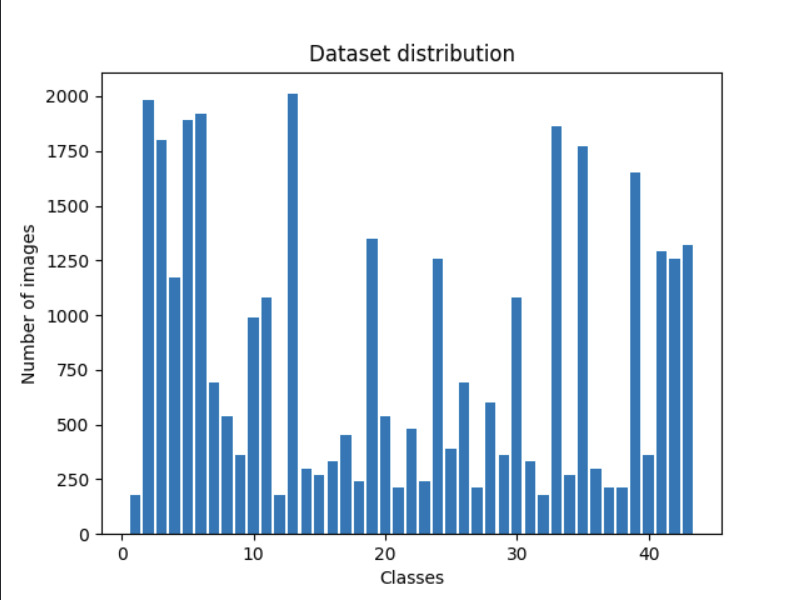
\includegraphics[width=\linewidth,trim=4 4 4 4,clip]{images/distribution.jpeg}
  \caption{Raspodijela dataseta po razredima.}
\end{figure}
\pagebreak
\section{Pretprocesiranje}
Pretprocesiranje ulaznog skupa podataka obavlja se pomoću sljedećeg bloka programskog koda:
\begin{lstlisting}[language=Python]
import cv2


def preprocess(image):
    image = cv2.cvtColor(image, cv2.COLOR_BGR2GRAY)
    image = cv2.equalizeHist(image)
    image = image / 255
    return image
\end{lstlisting}

S obzirom da za prepoznavanje zadanog skupa prometnih znakova nije potrebna informacija o boji, svaka ulazna slika se pretvara u \emph{grayscale}.
Također kako bi \emph{dataset} bio što iskoristiviji, slikama se povećava kontrast tehnikom histogramskog izjednačavanja. Metoda izjednačavanja histograma (HE) je široko korištena tehnika pretprocesiranja slike i svrstava se u kategoriju korekcija svjetline. 
Primjeri primjene HE su poboljšanje medicinskih slika, znanstvenih fotografija, povijesnih slika i sonarskih slika. Histogramsko izjednačavanje se također koristi i za poboljšanje kontrasta slike u digitalnim slikama. 
Navedeni učinci se postižu učinkovitim distribuiranjem najčešćih vrijednosti intenziteta. To omogućuje da povećamo kontrast na lokalnim dijelovima slike s lošim kontrastom \citep{9642082}.
Tehnikom histogramskog izjednačavanja se efektivno proširuje raspon vrijednosti intenziteta s ciljem povećanja kontrasta. Ova tehnika se često koristi i na slikama koje su imale loše osvijetljenje.
Naposlijetku vrijednosti svakog piksela slike se normaliziraju na vrijednost iz skupa [0, 1]. Navedenim postupcima pretprocesiranja se pospješuje brzina i učinkovitost treniranja modela.
\begin{figure}[h!]
  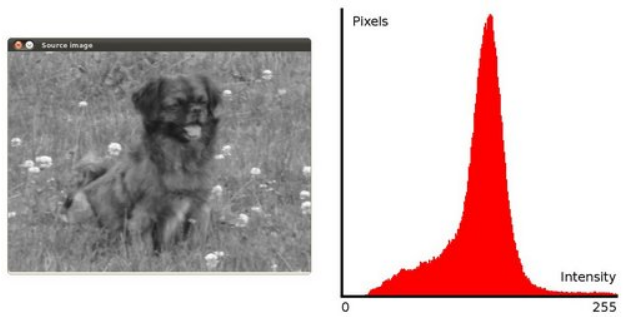
\includegraphics[width=\linewidth,trim=4 4 4 4,clip]{images/hist1.png}
  \caption{Primjer slike prije histogramskog izjednačavanja i odgovrajući histogram.}
  \source{\url{https://docs.opencv.org/3.4/d4/d1b/tutorial_histogram_equalization.html}}
\end{figure}
\begin{figure}[h!]
  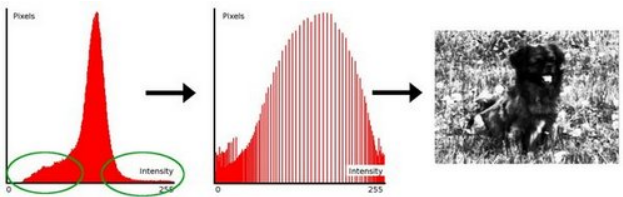
\includegraphics[width=\linewidth,trim=4 4 4 4,clip]{images/hist2.png}
  \caption{Primjer slike nakon histogramskog izjednačavanja i odgovrajući histogram.}
  \source{\url{https://docs.opencv.org/3.4/d4/d1b/tutorial_histogram_equalization.html}}
\end{figure}
\pagebreak
\clearpage
\section{Augmentacija skupa podataka}
Kako bi iskoristivost skupa podataka za treniranje bila maksimizirana korištena je augmentacija nad ulaznim skupom.
Augmentacija se provodi u sljedećem bloku programskog koda:
\\
\begin{lstlisting}[language=Python]
from keras.preprocessing.image import ImageDataGenerator


def augment():
    data_gen = ImageDataGenerator(width_shift_range=0.1,
                                  height_shift_range=0.1,
                                  zoom_range=0.2,
                                  shear_range=0.1,
                                  rotation_range=10)
    return data_gen
\end{lstlisting}

Gore prikazana funkcija koristi \code{ImageDataGenerator} funkciju iz
\\
\code{keras.preprocessing.image} modula. Uz navedene argumente ova metoda proširuje \emph{dataset} tako što svaku sliku
\begin{itemize}
	\item  Nasumično pomiče horizontalno uz maksimalni faktor od 10\% širine slike
	\item  Nasumično pomiče vertikalno uz maksimalni faktor od 10\% visine slike
	\item  Uvećava sliku u rasponu od 0\% do 20\%
	\item  Posmiče slike uz maksimalni kut posmaka od 10\textdegree 
	\item  Rotira sliku uz maksimalni kut rotacije od 10\textdegree
\end{itemize}
\begin{figure}[h!]
  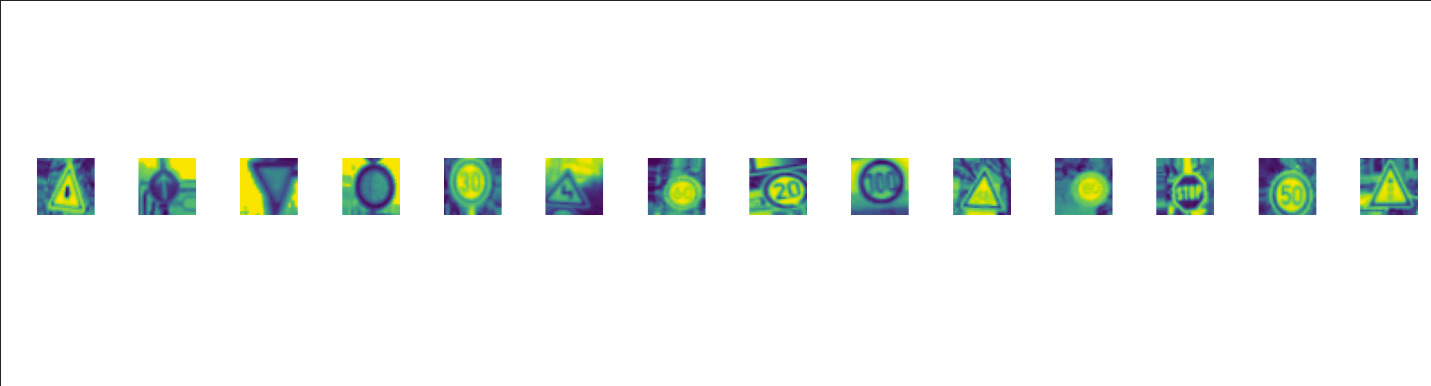
\includegraphics[width=\linewidth,trim=4 4 4 4,clip]{images/image-augmentation.jpeg}
  \caption{Prikaz augmentiranih slika.}
\end{figure}

\section{Treniranje modela}
Model strojnog učenja korišten za izradu ovog rada zasniva se na Keras API-u.
Sastoji se od jedanaest slojeva i reprezentiran je sljedećim isječkom Python koda:
\begin{lstlisting}[language=Python]
from keras.models import Sequential
from keras.layers import Dense
from keras.layers import Dropout, Flatten
from keras.layers.convolutional import Conv2D, MaxPooling2D


def learning_model(classes_len):

    model = Sequential()
    model.add((Conv2D(60, (5, 5), input_shape=(32, 32, 1),  activation='relu')))
    model.add((Conv2D(60, (5, 5), activation='relu')))
    model.add(MaxPooling2D(pool_size=(2, 2)))

    model.add((Conv2D(30, (2, 2), activation='relu')))
    model.add((Conv2D(30, (2, 2), activation='relu')))
    model.add(MaxPooling2D(pool_size=(2, 2)))
    model.add(Dropout(0.5))

    model.add(Flatten())
    model.add(Dense(500, activation='relu'))
    model.add(Dropout(0.5))
    model.add(Dense(classes_len, activation='softmax'))

    model.compile(optimizer='adam', loss='categorical_crossentropy', metrics=['accuracy'])
    return model
\end{lstlisting}

Prvi sloj je ulazni sloj neuronske mreže koji prima \emph{tensor} oblika (32, 32, 1), odnosno brojčanu reprezentaciju slike veličine 32*32 piksela s jednim kanalom (\emph{grayscale}). Zatim slijedi Conv2D sloj od 60 filtera veličine 5x5 piksela.
Konvolucijski slojevi neuronske mreže povezuju uzorke na manjim lokalnim regijama sloja s uzorcima koji se pojavljuju na korespondirajućim regijama iz viših slojeva čime se eliminira potreba za stvaranjem potpune povezanosti među slojevima \citep{8308186}.
Korištenjem nekolicine pojednostavljenja konvolucijski slojevi smanjuju broj stvorenih veza i za nekoliko redova veličine.\citep{turner2014lecture}
Sloj koristi ReLU aktivacijsku funkciju, odnosno zglobnicu definiranu formulom: \begin{align*} &ReLU(x)= max(0,x)\\ &\frac{d}{dx}(x)\ = \{1\ if\ x>0;\ 0\ otherwise\} \end{align*}
Glavna prednost ove aktivacije je što za ulaz 0, uvijek vraća 0, što nije slučaj kod nekih zasićenih funkcija poput \emph{tanh} i \emph{sigmoid} funkcija. Ovakvo ponašanje zasićenih funkcija može naštetiti treniranju modela.
Treći, peti i šesti slojevi modela imaju identičnu zadaću kao i prvi te se stoga ne razmatraju detaljnije.
Četvrti sloj je MaxPooling2D sloj, točnije agregacijski sloj. Zadaća agregacijskih slojeva je smanjivanje reprezentacije ulaza. Agregacijski sloj korišten u ovom modelu koristi prozor veličine 2*2 piksela te od te četiri vrijednosti uzima isključivo najveću.
Ovim postupkom se pospješuje generalizacija modela i suzbija se mogućnost stvaranja prenaučenog modela. Isto tako čini model robusnijim na translacije i pomake. Dodatni benefit se očituje i u performansama modela, zbog smanjene dimenzionalnosti računalni sustav vrši manje matričnih proračuna
što pak pospješuje brzinu učenja modela. U kontekstu smanjenja prenaučenosti i povećanja generalizacije modela koriste se i Dropout slojevi čija je zadaća nasumično isključivanje zadanog postotka ulaznih neurona kako bi se smanjio njihov individualni utjecaj.
Flatten sloj služi za pretvaranje višedimenzionalnih karakterističnih mapa u jednodimenzionalni vektor kako bi se omogućilo povezivanje sa slojevima potpuno povezane mreže. Konkretno, ako su ulazne karakteristične mape višedimenzionalne, poput 2D mapa dobivenih na izlazima konvolucijskih slojeva, 
Flatten sloj će izravnati te mape u jedan vektor, čime se gube prostorne informacije, ali se omogućuje dovođenje izlaza iz prethodnog sloja na ulaz potpuno povezanih slojeva koji očekuju jednodimenzionalne ulaze. 
Flatten sloj, dakle, osigurava da izlaz prethodnih slojeva bude u obliku pogodnom za obradu u potpuno povezanim slojevima, gdje svaki element vektora predstavlja značajku koju će mreža koristiti kako bi razriješila zadaće klasifikacije, ili u drugim primjenama regresije.
Dense slojevi, odnosno potpuno povezani slojevi povezuju sve ulazne jedinice (neurone) s izlaznim jedinicama u prethodnom sloju.
Dense slojevi su često korišteni kao završni slojevi u neuronskim mrežama za klasifikaciju. Izlazi posljednjeg Dense sloja obično predstavljaju vjerojatnosti različitih klasa u problemu klasifikacije, a aktivacijska funkcija koja se koristi na posljednjem sloju je obično softmax funkcija koja pretvara izlaze u vjerojatnosti.
\pagebreak
Aktivacijska funkcija korištena u posljednjem sloju je upravo gore spomenuti softmax.
Softmax funkcija je definirana formulom: 
\begin{eqnarray}
\sigma(y_{i}) = \left(\frac{e^{y_{i}}}{ \sum\limits_{j} e^{y_{j}}}\right)
j = 1,...,n
\end{eqnarray}

Motivacija za odabir ove aktivacijske funkcije je njena učinkovitost kad se kao metoda izračuna pogreške, odnosno funkcija gubitka koristi kategorička unakrsna entropija \emph{(categorical crossentropy)} \citep{dunne1997pairing}.
Dunne i Campbell su u svom radu "On the pairing of the softmax activation and cross-entropy penalty functions and the derivation of the softmax activation function", potaknuti hipotezom da postoji prirodno uparivanje te dvije funkcije pokušali empirijski potvrditi tu pretpostavku te su ostvarili izrazito pozitivne rezultate. 

Model koristi Adaptive Moment Estimation optimizator, skračeno Adam. Ovaj optimizator je zapravo proširenje metode stohastičkog gradijentnog spusta.
Adam kombinira prednosti dviju drugih tehnika optimizacije: AdaGrad, koja prilagođava stopu učenja za svaki parametar na temelju njihovih prošlih gradijenata, i RMSprop, koji koristi eksponencijalno smanjujuće promjenjive prosjeke kvadrata povijesnih gradijenata.
Osnovna ideja iza Adama je održavanje prilagodljive stope učenja za svaki parametar estimirajući prvi moment (srednju vrijednost) i drugi moment (necentriranu varijancu) gradijenata. Ta prilagodba pomaže procesu optimizacije da brže i stabilnije konvergira.\citep{kingma2014adam}

Treniranje modela se provodilo kroz 30 epoha, no praćenjem podataka o preciznosti modela postaje jasno da se model mogao trenirati i značajno kraće.
U priloženim grafikonima se jasno vidi da već nakon 10 do 15 epoha model postiže preciznost veću od 95\% na skupu za treniranje i preciznost veću od 99\% na skupu za validaciju.
\begin{figure}[h!]
  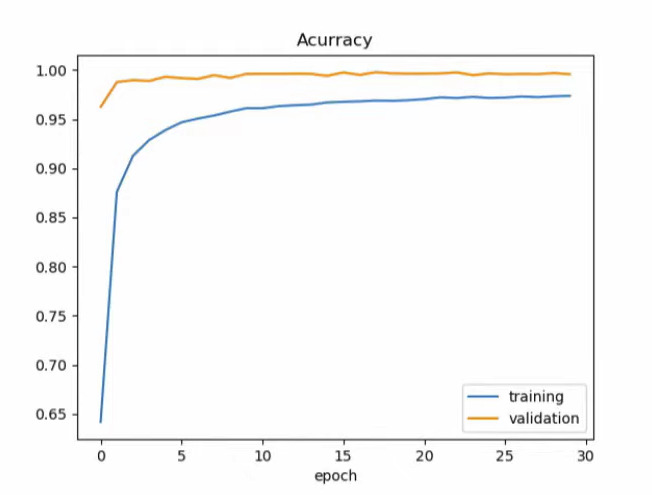
\includegraphics[width=\linewidth,trim=4 4 4 4,clip]{images/acc_plot.jpeg}
  \caption{Prikaz vrijednosti izračunate preciznosti kroz epohe.}
  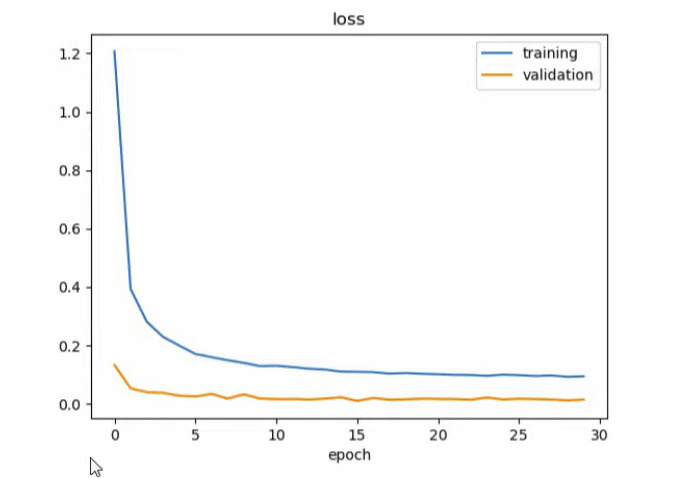
\includegraphics[width=\linewidth,trim=4 4 4 4,clip]{images/loss_plot.jpeg}
  \caption{Prikaz vrijednosti funkcije gubitka kroz epohe.}
\end{figure} 

\pagebreak
\section{Testna aplikacija}
Kako bi se testirala učinkovitost modela, razvijena je jednostavna testna skiripta u programskom jeziku Python. Skripta uključuje  \emph{web-kameru} računala, učitava istrenirani model te povezuje naziv svakog razreda s njegovim indeksom pomoću riječnika.
\\Primjerice:
\begin{lstlisting}[language=Python]
class_names = {
    0: 'Speed Limit 20 km/h',
    1: 'Speed Limit 30 km/h',
    ...
}
\end{lstlisting}

Zatim u beskonačnoj petlji učitava sliku s \emph{web-kamere}, pretprocesira tu sliku, vrši predikciju pomoću istreniranog modela. Ukoliko je vjerojatnost s kojom je model predvidio da se na slici nalazi neki znak veća od unaprijed zadanog praga na zaslonu se ispisuje naziv
znaka te vjerojatnost s kojom model klasificira sliku znaka u pretpostavljeni razred. Naprotiv, ukoliko je vjerojatnost niža od zadanog praga ispisuje se samo prikladna poruka da model ne prepoznaje znak na slici.
\\Uz jasna ograničenja koje ovaj model testne aplikacije posjeduje (nedostatak grafičkog sučelja, uporaba ugrađene kamere umjesto zasebne kamere ili senzora), aplikacija ipak može poslužiti kao kvalitetni pokazatelj učinkovitosti i brzine kojom model vrši predikcije i daje finalni rezultat. 
%TODO: slika izgleda ispisa


\section{Ispitivanje sustava}
Testiranje rada cjelokupnog sustava je provedeno u dvije faze. Prvo se nadzirala klasifikacijska preciznost na skupu podataka za validaciju, rezultati dobiveni u toj fazi ispitivanja su navedeni u poglavlju 3.4. Druga faza testiranja sustava je bazirana na ispitivanju prikladnosti sustava za provođenje klasifikacije u stvarnom vremenu.
Pripremljeno je 42 primjera prometnih znakova. Svaki od tih primjera je podvrgnut manipulacijama svjetline, orijentacije i kontrasta. 
\begin{figure}[h!]
  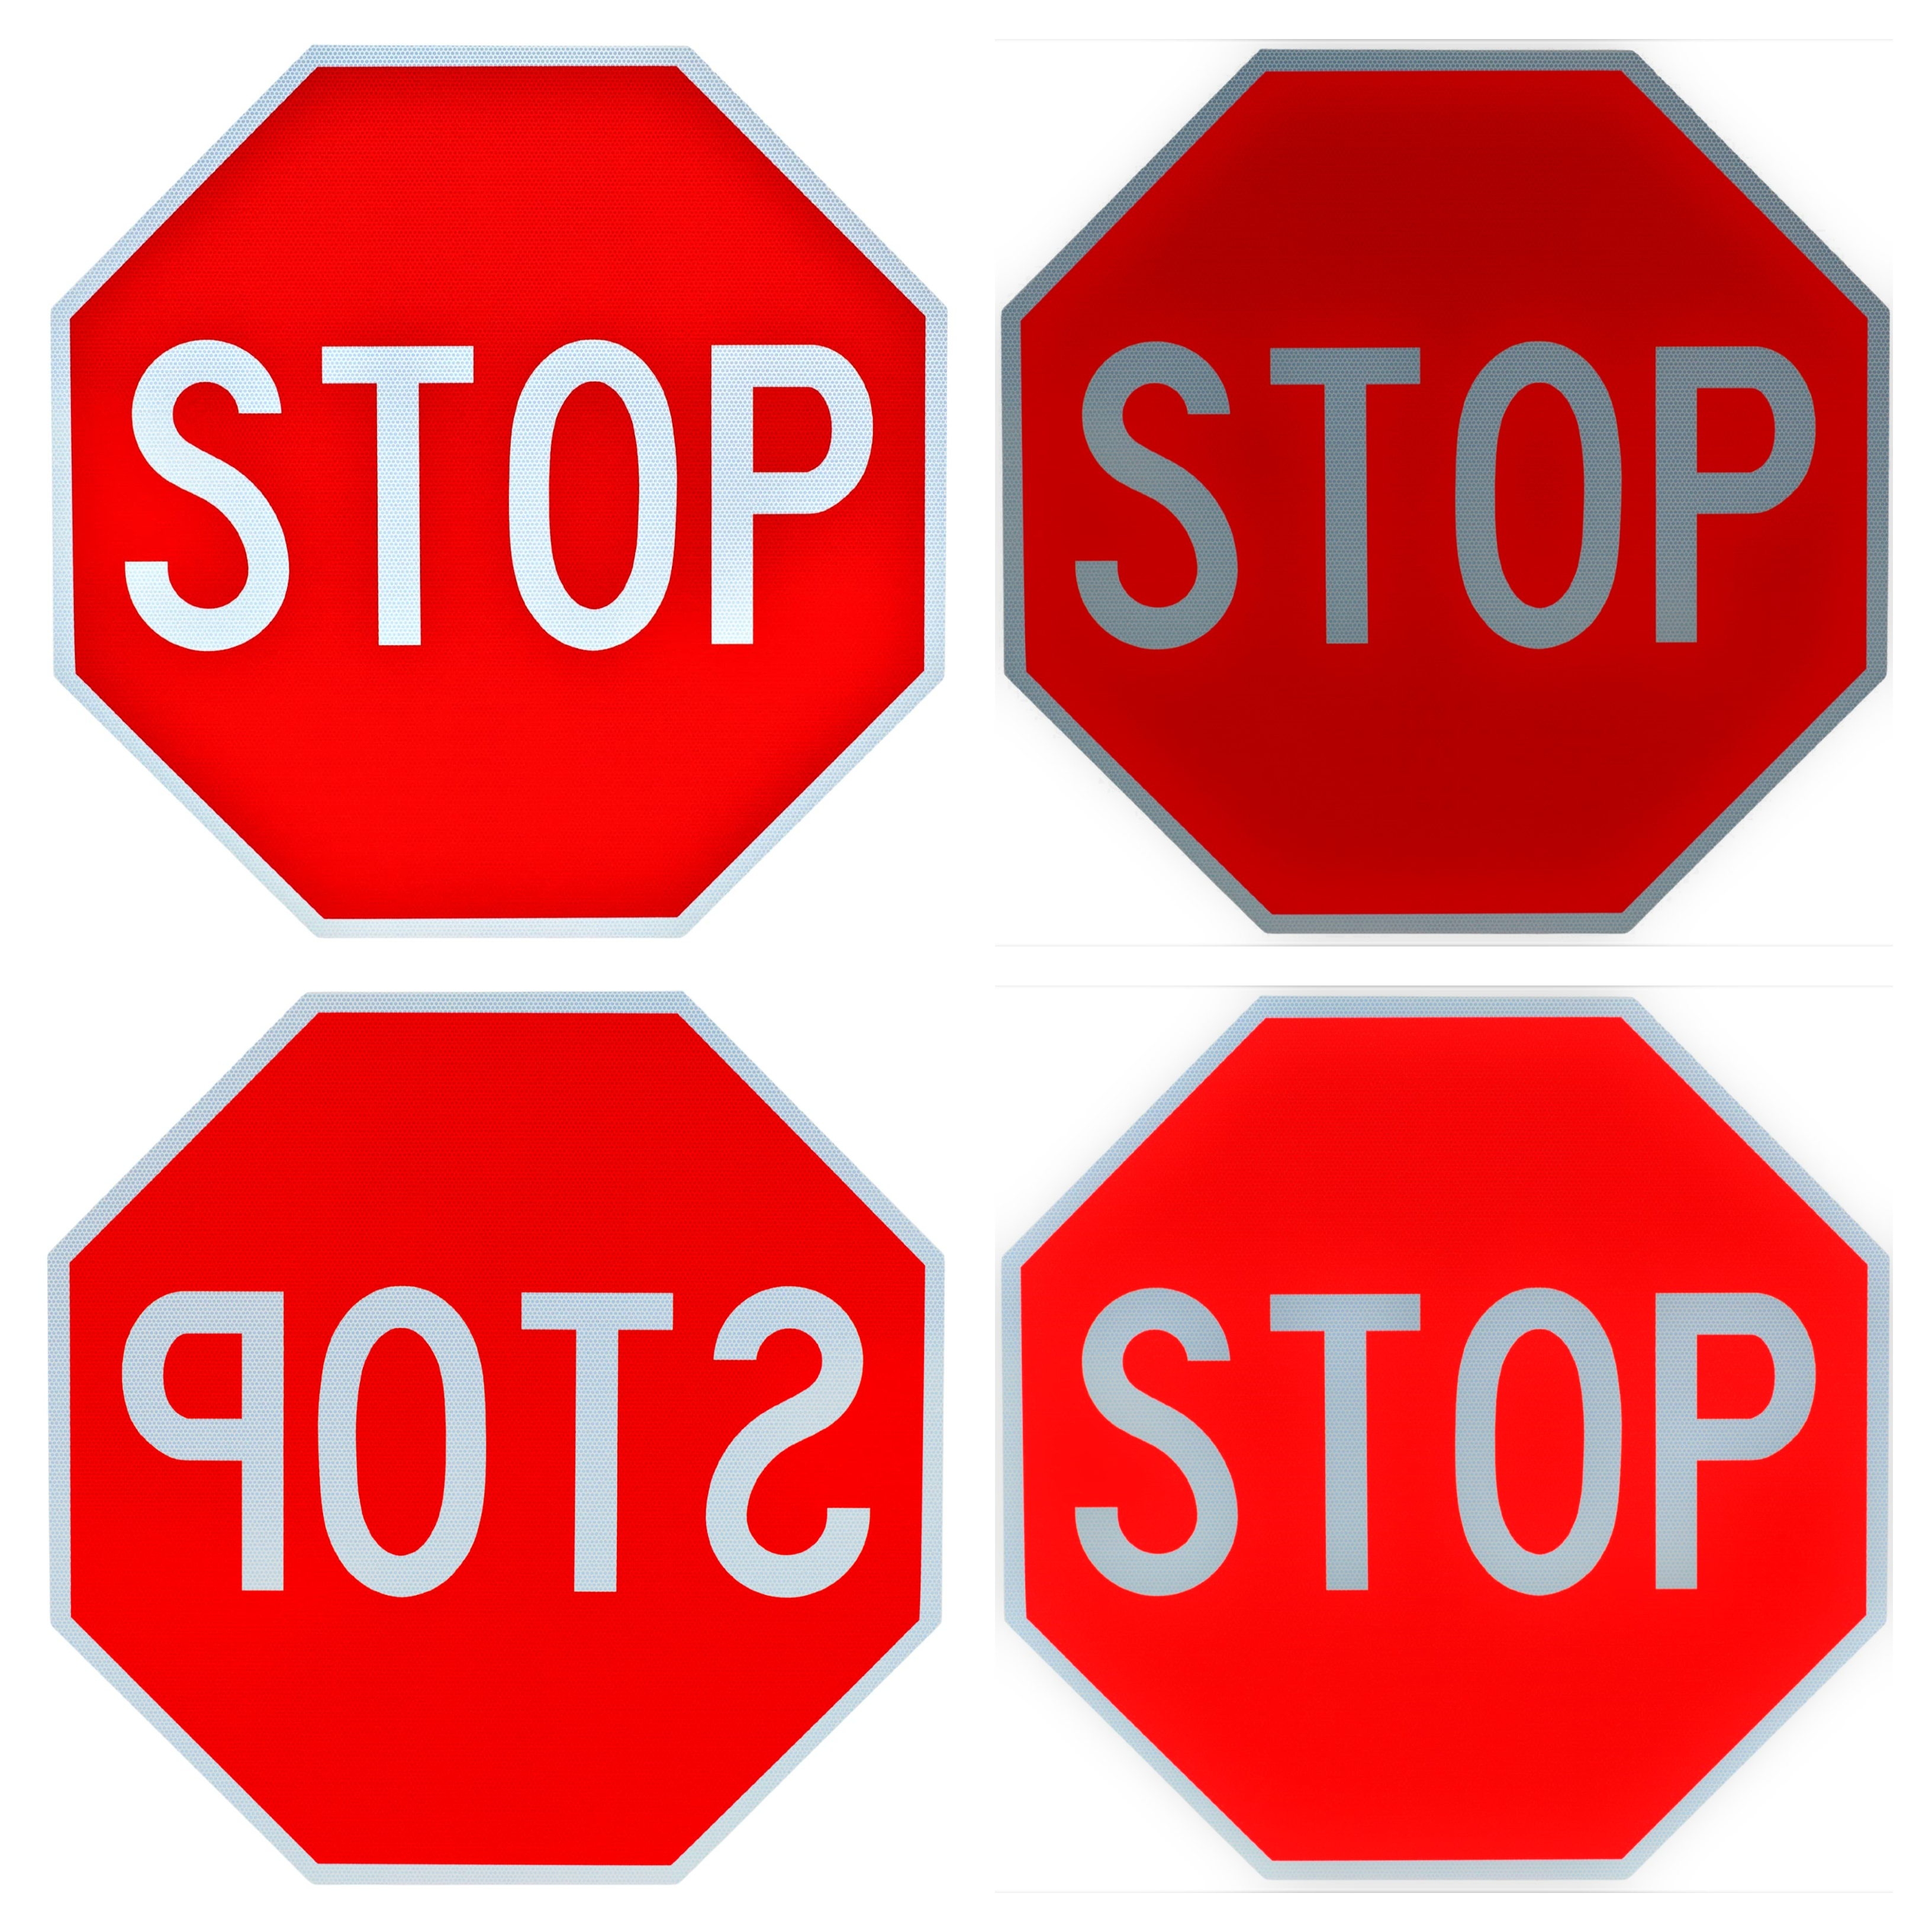
\includegraphics[width=\linewidth,trim=4 4 4 4,clip]{images/stop_test.jpg}
  \caption{a) izvorna slika
b) primjer smanjene svjetline
c) primjer zrcaljena po vertikalnoj osi
d) primjer povećanog kontrasta
}
\end{figure} 

Pripremljeni materijali su postavljeni ispred \emph{web-kamere} uz dva različita stupnja ambijentalnog osvijetljenja (potpuno svijetla prostorija i polumračna prostorija). Prilikom testiranja se pokazala snažna ovisnost između performansi modela za pojedini primjer i njegove zastupljenosti u skupu podataka za treniranje.
Promjene svjetline i kontrasta su na točnost klasifikacije djelovale s minimalnim utjecajem, no zrcaljenje primjera je za primjere koji su u skupu podataka za treniranje bili manje zastupljeni je uzrokovalo značajni pad u točnosti. Znakove koji su u \emph{datasetu} bili zastupljeni s 500 ili više primjera
je model klasificirao ispravno u svim uvjetima sa stopom sigurnosti u klasifikacijsku odluku većom ili jednakom od 95\%. Znakove zastupljene s manje od 500, ali više od 250 primjera je ispravno klasificirao u svim uvjetima sa stopom sigurnosti između 92\% i 97\%. Performanse modela su bile najgore za znakove koji su se u \emph{datasetu}
bili zastupljeni s 250 primjera ili manje. Pri ispitivanju takvih primjera su zrcaljeni primjeri bili prepoznati u tek nešto više od 75\% slučajeva. Bitno je napomenuti da su primjeri koji bi zrcaljeni prezentirali neki drugi znak bili preskočeni u ovoj fazi ispitivanja.

\chapter{Rezultati}
Početni zahtjevi koji su stavljeni pred sustav su se ponajviše bazirali na brzinu i točnost klasifikacije. Cilj je bio ostvariti točnu klasifikaciju u čim kraćem vremenu.
Rezultati klasifikacije postignuti uporabom kreiranog modela su izrazito povezani s veličinom podskupa skupa podataka za učenje koji je sadržavao primjere klasificirane klase. Tako primjerice za znakove koji su u \emph{dataset-u} bili reprezentirani s više od 1000 primjera model primjere 
u velikoj većini slučajeva klasificira ispravno i sa sigurnošću većom ili jednakom od 99\%. Primjere znakova koji su bili znatno manje zastupljeni u skupu podataka za učenje model i dalje, uglavnom, ispravno klasificira no sa znatno manjom sigurnošću, tek nešto iznad zadanog praga od 90\% sigurnosti.
Vrijedi napomenuti da je navedeni prag upravo uveden kako bi se čim više smanjio broj lažno pozitivnih klasifikacija koje je model radio. Prilikom testiranja modela u uvjetima u kojima je klasifikacijski prag sigurnosti bio niži od 75\% model je često klasificirao ljudska lica, vozila i ostale
primjere koji nisu pripadali klasi prometnh znakova. Brzina s kojom model donosi odluke je također dovoljna za klasifikaciju u stvarnom vremenu, odnosno red veličine nekoliko desetaka milisekundi.
Naučeni model koji se koristi u klasifikaciji je poprilično agnostičan prema poremečajima osvjetljenja i kontrasta koji su uneseni tijekom ispitivanja sustava te uspješno klasificira čak i u takvim uvjetima.

\chapter{Budući rad}
Budući rad na ovom problemu bi uključivao implementaciju detekcije prometnih znakova na slici kako bi cjelokupni sustav bio što iskoristiviji u stvarnom svijetu. Nužno bi bilo uvesti i neku vrstu dediciranog senzora ili kamere koja bi imala dovoljne mogućnosti stabilizacije, 
rada u mraku i uvjetima smanjene vidljivosti (kiša, magla, snijeg...). Sljedeći korak bi bio treniranje modela na jačem \emph{hardware-u} kroz više epoha kako bi se pospiješila klasifikacija znakova. Posljednji koraci budućeg razvoja bi uključivali verzioniranje sustava za razna tržišta, primjerice
razvoj odvojenih verzija za tržište Sjedninjenih Američkih Država zbog razlike u standardu prometnih znakova u odnosu na europske standarde za koje je trenutna aplikacija prilagođena.

\chapter{Zaključak}
U ovom završnom radu predstavljene su primjene sustava za klasifikaciju prometnih znakova i izazovi koji se javljaju prilikom implementacije istih. Implementira se model strojnog učenja baziran na konvolucijskoj neuronskoj mreži i trenira se na GTRSB skupu podataka za učenje, 
a zatim se istrenirani model koristi za klasifikaciju fotografija prometnih znakova fotografiranih \emph{web-kamerom} prijenosnog računala. Ostvareni sustav demonstrira kako i model jednostavne arhitekture, sazdan od 11 slojeva, može učinkovito klasificirati prometne znakove.
Uzmemo li u obzir da se treniranje modela izvršavalo na ograničenom skupu podataka za treniranje i samo jednom CPU-u, zaključujemo da je čak i s ograničenim resursima moguće otvariti sustav za klasifikaciju koji je relativno otporan na poremećaje osvjetljenja, pomicanja kamere i poremećaje u kontrastu.
Ostvareni sustav primjere klasificira dovoljno brzo i precizno za demonstrativne primjene, no njegova primjena u stvarnim uvjetima bi bila izrazito ograničena bez dodavanja specijalizirane senzorike i sustava za detekciju. 

\begin{sazetak}
Rad opisuje jednu moguću implementaciju sustava za klasifikaciju prometnih znakova u stvarnom vremenu. Razrađuju se primjene i zahtjevi sustava, opisuju se ranija ostvarenja u tom području i definira se pristup rješenju problema klasifikacije.
Sustav klasificira prometne znakove uporabom jedne konvolucijske neronske mreže koja se sastoji od 12 slojeva. Za potrebe treniranja neuronske mreže korišteni su razni pristupi pretprocesiranja fotografija iz skupa podataka za učenje kako bi se povećao broj ulaznih podataka koje model 
ima na raspolaganju za učenje ali i učinio model otpornijim na poremečaje u osvjetljenju i kontrastu do kojih može doći na ulazu. Istrenirani model se koristi u testnoj aplikaciji koja konstantno uzima slike s  \emph{web-kamere} prijenosnog računala, zatim te slike pokušava klasificirati te ukoliko
s određenom sigurnošću uspije klasificirati fotografiju ispisuje rezultat na zaslon prijensnog računala.

\kljucnerijeci{Klasifikacija, računalni vid, strojno učenje, duboko učenje, duboke neuronske mreže, konvolucijske neuronske mreže, prometni znakovi, promet, DNN, CNN, CV, ML}
\end{sazetak}
\pagebreak
\engtitle{Traffic sign classification}
\begin{abstract}
The paper describes a possible implementation of a real-time traffic sign classification system. 
The applications and requirements of the system are discussed, previous achievements in the field are described, and an approach to solving the classification problem is defined.
Created system classifies traffic signs using a single convolutional neural network consisting of 12 layers. 
Various preprocessing approaches were used to augment the training dataset, increasing the number of input data available for the model to learn from and making the model more robust to disturbances in lighting and contrast that may occur at the input. 
The trained model is used in a test application that continuously captures images from a laptop's webcam, attempts to classify those images, and if successful with a certain confidence, displays the result on the laptop's screen.

\keywords{Classification, Computer Vision, Machine Learning, Deep Learning, Deep Neural Networks, Convolutional Neural Networks, Traffic Signs, Traffic, DNN, CNN, CV, ML}

\end{abstract}


\bibliography{literatura.bib}
\bibliographystyle{fer}

\listoffigures


\end{document}
